 \documentclass[../analysisII_notes.tex]{subfiles}
\begin{document}
\section{Aula 13 - 28 de Abril, 2025}
\subsection{Motivações}
\begin{itemize}
	\item O Teorema de Lebesgue.
\end{itemize}
\subsection{O Teorema de Lebesgue.}
Nesta aula, finalmente iremos mostrar a caracterização completa de quais funções são Riemann-Integráveis em um intervalo \([a, b]\). Para isso, utilizaremos todo o nosso aprendizado até o momento - desde o básico das integrais às propriedades de conjuntos de medida nula.
\hypertarget{lebesgue_theorem}{\begin{theorem*}[O Teorema de Lebesgue]
		Para que uma função limitada \(f:[a, b]\rightarrow \mathbb{R}\) seja integrável, é necessário e suficiente que o conjunto D, caracterizado pelos pontos de descontinuidade da f em seu domínio, tenha medida nula.
	\end{theorem*}}
Em particular, pela caracterização dos conjuntos de medida nula, já ganhamos que, tanto os conjuntos finitos de descontinuidades de uma função, quanto os que forem enumeráveis, ainda assim não impedem que ela seja integrável.
\begin{proof*}
	\hypertarget{next_class_13}{Prova da condição} ser necessário (\(\Rightarrow \))): primeiro, observemos que, pela continuidade em um ponto em termos da oscilação em um ponto p,
	\[
		D = \{p\in [a, b]: \omega(f; p)>0\};
	\]
	em segundo lugar, perceba também que, se para todo j natural colocarmos
	\[
		D_{j} \coloneqq \biggl\{p\in [a, b]: \omega (f; p) > \frac{1}{j}\biggr\},
	\]
	então
	\[
		D = \bigcup_{j=1}^{\infty}D_{j}.
	\]

	Com efeito, se um ponto p pertence a \(D_{j}\) para algum j, então a oscilação de f em p neste conjunto ainda assim é positivo, garantindo que
	\[
		D_{j} \subseteq D \quad \forall j\in \mathbb{N} \Rightarrow \bigcup_{j=1}^{\infty}D_{j} \subseteq D.
	\]
	Por outro lado, se p for um ponto em D, vale que
	\[
		\omega (f; p) > 0,
	\]
	donde segue que existe um certo índice \(j_{0}\) a partir do qual
	\[
		\frac{1}{j_{0}}<\omega (f; p) \Rightarrow p\in D_{j_{0}}.
	\]
	Logo, tendo encontrado pelo menos um membro da união no qual os p's de D estão, segue que
	\[
		D \subseteq \bigcup_{n=1}^{\infty}D_{j}.
	\]

	Ademais, para provar que a medida de D é nula, basta provar que a medida de cada um dos membros da coleção enumerável \(\{D_{j}\}_{j\in \mathbb{N}}\) tem medida nula.
	Com efeito, fixemos algum j natural; mostraremos que a medida de \(D_{j}\) é nula, o que consiste em encontrar uma cobertura enumerável por intervalos fechados tal que a soma dos comprimentos dele possa ser quão pequena desejarmos.

	Para tal, tome \(\varepsilon > 0\) qualquer; usando a integrabilidade de f dentro do intervalo \([a, b]\) e o \hyperlink{integrability_conditions}{\textit{Critério de Riemann}}, deve existir uma partição
	\[
		\mathcal{P}: a = t_{0} < t_1 < \dotsc <t_{n} = b
	\]
	com
	\[
		\sum\limits_{i=1}^{n}\omega_{i}(t_{i}-t_{i-1}) < \frac{\varepsilon }{j}.
	\]
	Nessas condições, sejam
	\[
		[t_{i_{1}-1}, t_{i_{1}}],\; [t_{i_{2}-1}, t_{i_{2}}], \dotsc , [t_{i_{r}-1}, t_{i_{r}}],
	\]
	os intervalos de \(\mathcal{P}\) que contêm algum ponto de \(D_{j}\) em seu interior, isto é,
	\[
		(t_{i-1}, t_{i})\cap D_{j} \neq\emptyset \Rightarrow i\in \{i_{1}, \dotsc , i_{r}\}.
	\]
	\begin{figure}[H]
		\begin{center}
			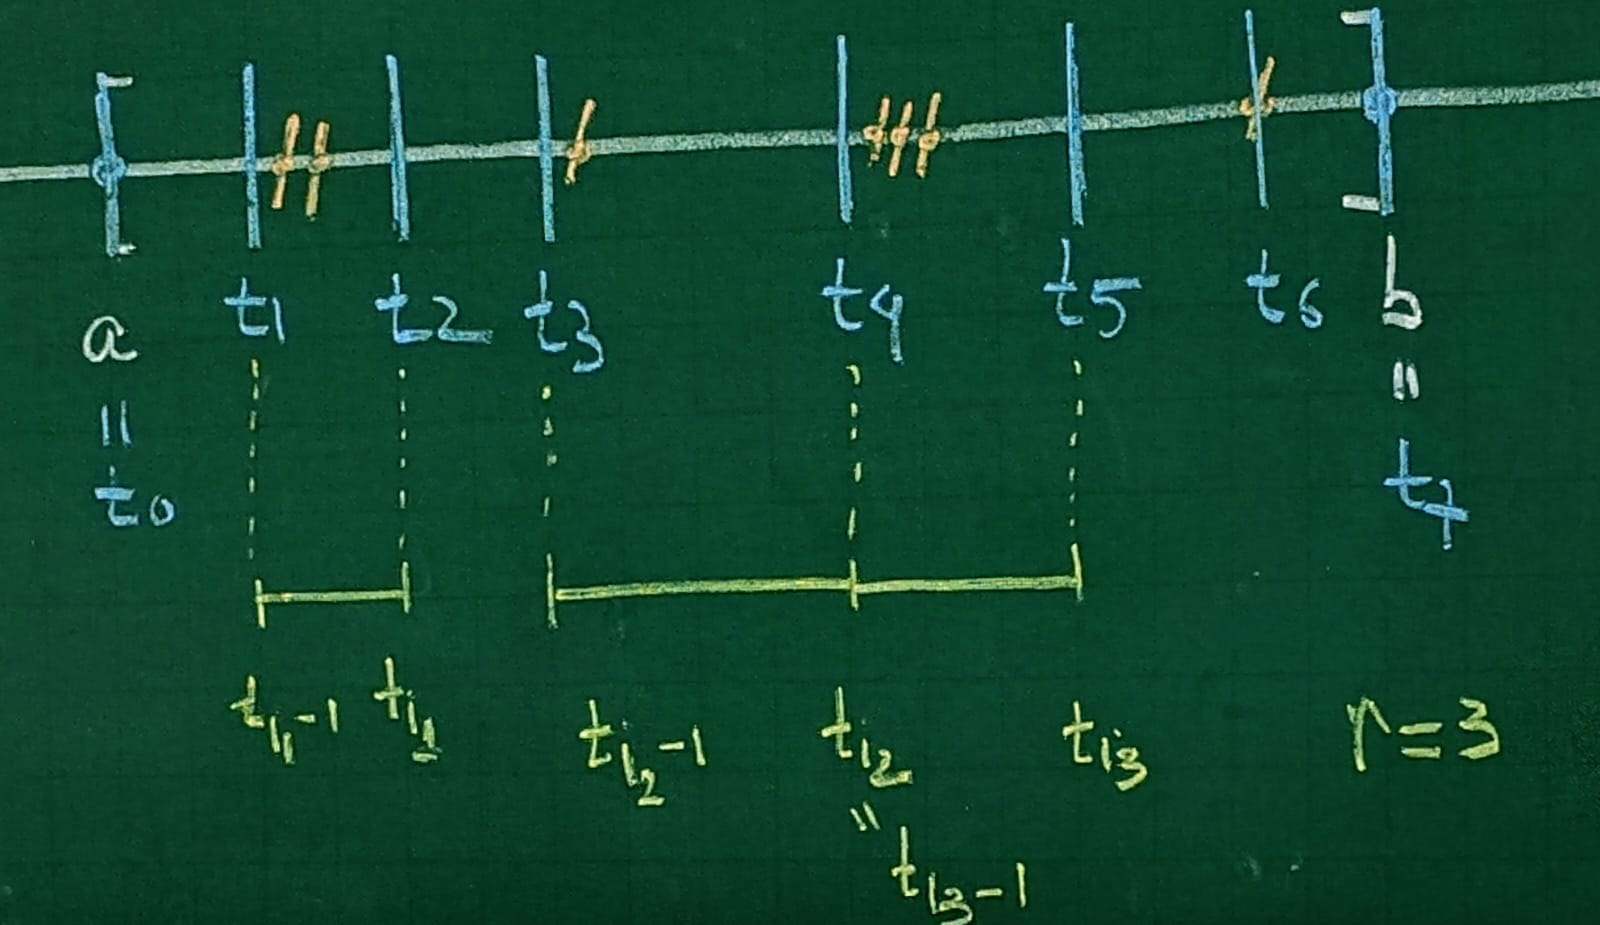
\includegraphics[height=0.5\textheight, width=0.5\textwidth, keepaspectratio]{./Images/partition_13.png}
		\end{center}
		\caption{escolha dos intervalos subindexados de 1 até r da partição, pintados em amarelo. Note que nem todos os intervalos da partição em si contêm um ponto de \(D_{j}\) (os riscos laranjas) em seu interior - basta olhar para \([t_{2}, t_{3}]\). Com base nisso, r vale 3 aqui!}
		\label{part13}
	\end{figure}

	Note que, com essa seleção e com o j fixo do começo,
	\[
		\omega_{i_k} \geq \frac{1}{j},\quad \forall k=1, 2, \dotsc , r.
	\]
	Isto é verdade pois, pelas propriedades das oscilações pontuais de funções, elas sempre serão menores do que a oscilação da função no intervalo do qual os pontos são interiores:
	\[
		p\in \mathrm{Int}(I) \Rightarrow \omega(f; p) \leq \omega (f; I).
	\]
	Daí, como \([t_{i_{k}-1}, t_{i_{k}}]\) contém um ponto p do conjunto \(D_{j}\) em seu interior, vale que
	\[
		\frac{1}{j}<\omega (f; p) \leq \omega (f; [t_{i_k-1, t_{i_k}}]) = \omega_{i_{k}}.
	\]
	Dessa forma,
	\begin{align*}
		\frac{\varepsilon }{j} > \sum\limits_{i=1}^{n}\omega_{i}(t_{i}-t_{i-1}) & \geq \sum\limits_{k=1}^{r}\omega_{i_{k}}(t_{i_k}-t_{i_{k}-1})                    \\
		                                                                        & > \frac{1}{j}\sum\limits_{k=1}^{r}(t_{i_{k}}-t_{i_{k}-1})                        \\
		                                                                        & \Rightarrow \sum\limits_{k=1}^{n}\ell ((t_{i_{k}-1}, t_{i_{k}})) < \varepsilon .
	\end{align*}

	Em resumo, o argumento mostrou que ou a descontinuidade é um dos extremos da partição (que já irá caracterizar um conjunto finito, pois a partição assim o é), ou existe uma cobertura finita por intervalos de tamanhos pequenos como desejarmos cobrindo a partição, ou seja, existem \(J_{0}, \dotsc , J_{n}\) com
	\[
		\mathcal{P}\subseteq \bigcup_{\ell =0}^{n}J_{\ell}:\; \sum\limits_{\ell =0}^{n}\ell (J_{\ell }) < \varepsilon  \Rightarrow D_{j} \subseteq \biggl(\bigcup_{\ell =0}^{n}J_{\ell}\biggr)\cup \biggl(\bigcup_{k=1}^{r}I_{i_{k}}\biggr)\;\&\; \sum\limits_{\ell =0}^{n}\ell (J_{\ell}) + \sum\limits_{k=1}^{r}\ell (I_{i_{k}}) < 2\varepsilon.
	\]
	Portanto,
	\[
		m(D_{j}) - 0,
	\]
	como queríamos.

	Quanto à condição ser suficiente (\(\Leftarrow )\)): supondo que f tem medida nula, dado um número positivo \(\delta_{1}\), existe uma sequência de intervalos
	\[
		I_1, I_2, \dotsc , I_n, \dotsc
	\]
	de intervalos abertos que cobrem \(D\) e cuja soma dos comprimentos é menor do que \(\delta_1\). Por outro lado, se p for um ponto do intervalo \([a, b]\), mas não de D, então dado outro número positivo \(\delta_2\), existirá outro \(\delta_p\) positivo tal que
	\[
		\omega (f; X_{\delta_{p}}) < \delta_{2},
	\]
	em que
	\[
		X_{\delta_{p}} \coloneqq [a, b]\cap [p-\delta_p, p+\delta_p].
	\]
	A desigualdade da oscilação de f em \(X_{\delta_p}\) é verdadeira pois
	\[
		0 = \omega (f; p) = \lim_{\delta \to 0^{+}}\omega (f; X_{\delta_{p}}).
	\]
	Diante de tudo isso, usando a denotação para cada ponto p que não é descontinuidade de f
	\[
		J_{p}\coloneqq (p-\delta_p, p+\delta_p),
	\]
	criamos uma cobertura aberta para o intervalo \([a, b]\) da forma
	\[
		[a, b]\subseteq \biggl(\bigcup_{i=1}^{\infty}I_{i}\biggr)\cup \biggl(\bigcup_{p\not\in D}^{}J_{p}\biggr)
	\]
	e, como \([a, b]\) é um conjunto compacto, podemos aplicar o \hyperlink{heine_borel}{\textit{Teorema de Heine-Borel/Borel-Lebesgue}} para extrair uma subcobertura finita:
	\[
		[a, b] \subseteq I_1\cup I_2\cup \dotsc \cup I_{n}\cup J_{p_1}\cup J_{p_2}\cup \dotsc \cup J_{p_{m}}.
	\]
	\begin{figure}[H]
		\begin{center}
			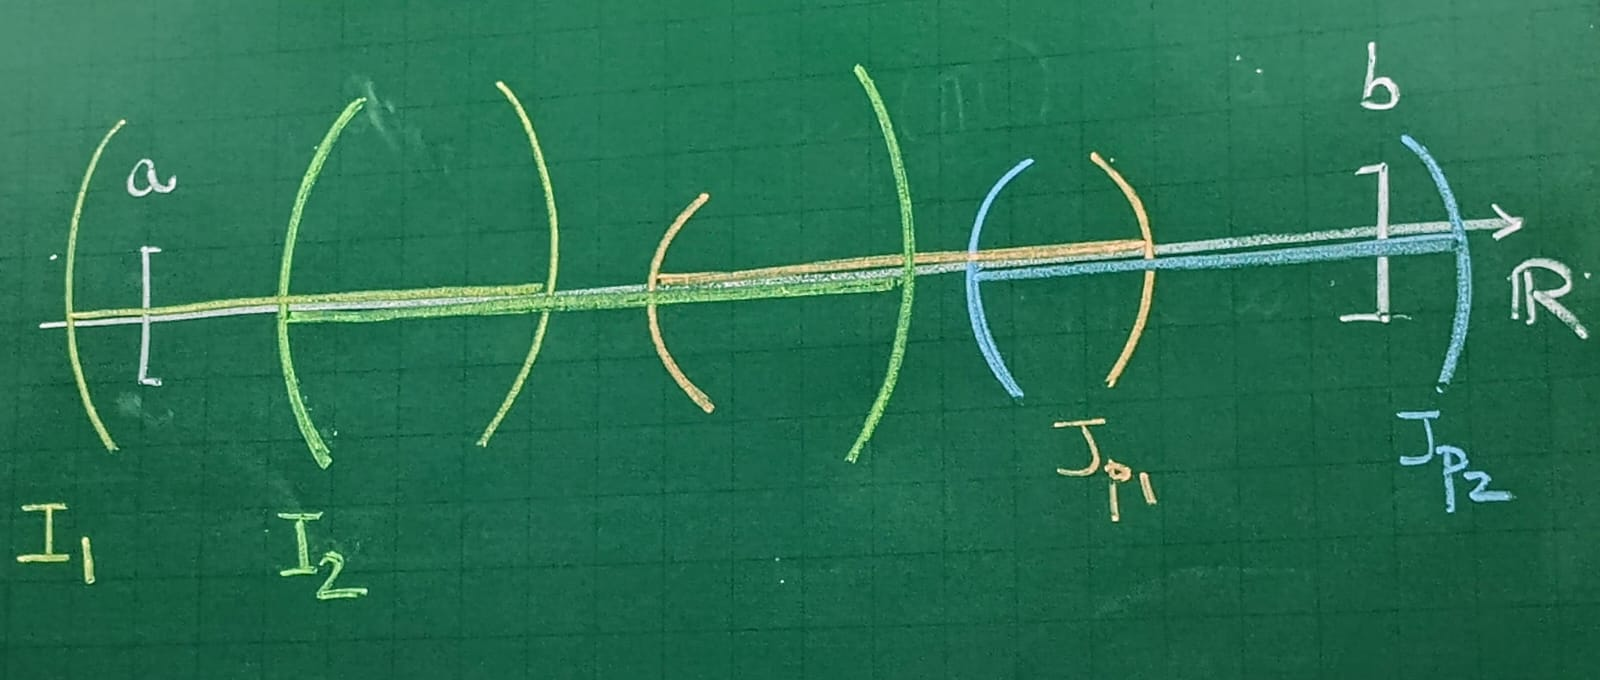
\includegraphics[height=0.5\textheight, width=0.5\textwidth, keepaspectratio]{./Images/covering_intervals_13.png}
		\end{center}
		\caption{separação de \([a, b]\) na união dos conjuntos \(I_{i}\) e \(J_{p}\).}
		\label{aa13}
	\end{figure}

	Nestas condições, seja \(\mathcal{P}\) a partição de \([a, b]\) formada por a e b e as extremidades dos \(I_{i}\)'s e \(J_{p_{j}}\)'s que estão em \([a, b]\). Vamos classificar os intervalos de \(\mathcal{P}\) em duas categorias: a categoria \(\alpha \), formada pelos subintervalos \([t_{i_{1}^{\alpha }-1}, t_{i_{1}^{\alpha }}], \dotsc , [t_{i_{r}^{\alpha }-1}, t_{i_{r}^{\alpha }}]\) de P que estão contidos no fecho de algum \(I_{i}\); e os \(\beta \), que são o que sobrou, denotados por \([t_{i_{1}^{\beta }-1}, t_{i_{1}^{\beta }}],\dotsc ,[t_{i_{s}^{\beta }-1}, t_{i_{s}^{\beta }}]\).
	Perceba que, se um intervalo é beta, então ele está contido no fecho \(J_{p_{j}}\) para algum \(J_{p_{j}}\), pois nenhuma extremidade, inferior ou superior, de intervalo \(\beta \) pode estar na união dos \(I_{i}\)'s. Logo, ela deve estar na união dos \(J_{p_{j}}\)'s, o que obriga, por definição de \(\mathcal{P}\), que o intervalo qeu a tem como extremidade esteja contido no fecho do \(J_{p_{j}}\) que o contém.

	\begin{figure}[H]
		\begin{center}
			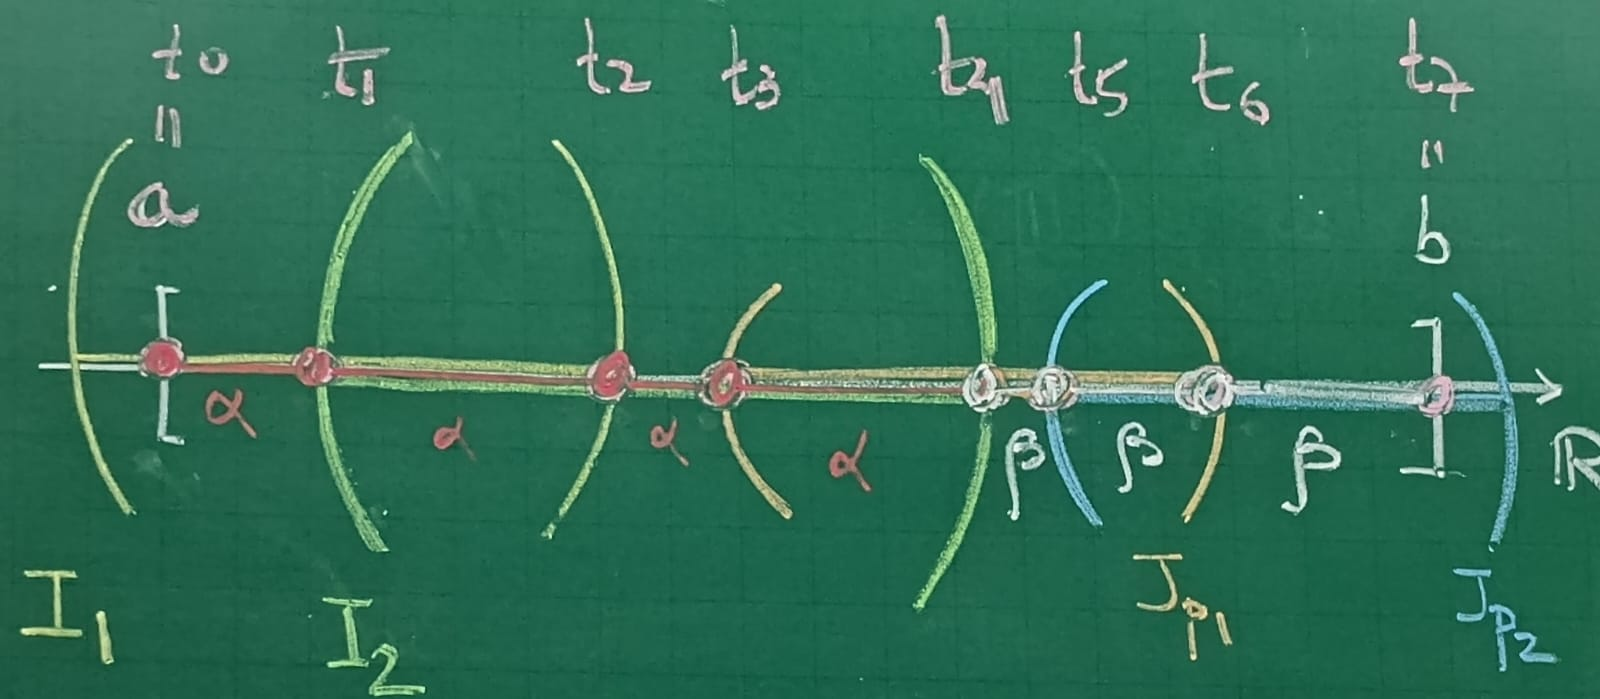
\includegraphics[height=0.5\textheight, width=0.5\textwidth, keepaspectratio]{./Images/classified_intervals_13.png}
		\end{center}
		\caption{separação dos intervalos nas classes \(\alpha \) e \(\beta \).}
		\label{classified13}
	\end{figure}

	(continua na próxima aula...).
\end{proof*}


\begin{tcolorbox}[
		skin=enhanced,
		title=Lembrete!,
		after title={\hfill Teorema de Heine-Borel},
		fonttitle=\bfseries,
		sharp corners=downhill,
		colframe=black,
		colbacktitle=yellow!75!white,
		colback=yellow!30,
		colbacklower=black,
		coltitle=black,
		%drop fuzzy shadow,
		drop large lifted shadow
	]
	O \hypertarget{heine_borel}{Teorema de Heine-Borel} pode ser enunciado como
	\begin{quote}
		``Um compacto no espaço euclideano n-dimensional é totalmente caracterizado (se, e somente se) como sendo fechado e limitado''
	\end{quote}
\end{tcolorbox}
\end{document}
